\section{Block Codes and Hamming Distance}\label{section_1.1}

\begin{definition}
  We define an \textbf{alphabet} to be an arbitrary finite set $Q$ of size $q$,
  whose elements we call \textbf{symbols}. Given some $n \in \Z^+$, we call
  elements of $Q^n=\underbrace{Q \times \dots \times Q}_{n\text{-times}}$
  \textbf{words} or \textbf{strings} in the alphabet.
\end{definition}

\begin{example}\label{example_1.1}
  \begin{enumerate}
    \item[(1)] The standard English alphabet
      \begin{align*}
        A B C D E F G H I J K L M N O P Q R S T U V W X Y Z \\
      \end{align*}
      is an alphabet of size $26$. A word in this alphabet can be the words
      ``DOG'' and ``COOKED'' as well as the word ``AFDAFDKAJFDAJFA''.

    \item[(2)] The \textbf{binary field} $\F_2=\{0,1\}$  (i.e. the finite field
      on two elements) is an alphabet of size $2$. Likewise, the
      \textbf{ternary field} $\F_3=\{0,1,2\}$ where $2 \equiv -1 \mod{3}$ is an
      alphabet of size $3$. We define the  \textbf{$q$-ary field} to be the
      finite field $\F_q$ on $q=p^r$ elements, where  $p,r \in \Z^+$ and $p$ is
      prime.

    \item[(3)] The fields $\R$ and $\C$ are not alphabets, since they are not
      finite sets; they are not even countable sets. The sets $\Q$ and $\Z$ and
      $\N$ are also not alphabets, they are countable, but not finite.
  \end{enumerate}
\end{example}

\begin{definition}
  Let $Q$ be an alphabet of size $q$. We define a \textbf{code} $C$ to be any
  non-empty collection of words in $Q$, and we call the elements of $C$
  \textbf{codewords}. If $C \subseteq Q^n$, then we call $C$ a  \textbf{block
  code} of \textbf{length} $n$.
\end{definition}

\begin{example}\label{example_1.2}
  \begin{enumerate}
    \item[(1)] The collection $\{\text{``DOG''}, \text{``CAT''},
      \text{``GOOSE''}\}$ is a code in the english alphabet, but it is not a
      block code. The code $\{\text{``DOG''}, \text{``CAT''},
      \text{``HAT''}\}$ is a block code of length $3$ in the english alphabet.

      \item[(2)] In $\F_2$, the codewords  $11001111$ and  $101011$ form a code
        in  $\F_2$ but not a block code. The codewords $11111$, $00000$,
        $11001$, and  $10101$ form a block code of length  $5$ in  $\F_2^5$.

      \item[(3)] We define the \textbf{$q$-ary repitition code} to be the image
        of the following map $\F_q \xrightarrow{} \F_q^n$ taking $i
        \xrightarrow{} (i, \dots, i)=i \dots i$. That is we take any symbol in
        $\F_q$ and repeat it $n$ times. This code is a block code of length $n$
        in $\F_q^n$.

      \item[(3)] Let $Q$ be any alphabet and  $C$ a block code of length  $n$.
        If $|C|=1$, then we say that $C$ is the  \textbf{trivial block code}, or
        the \textbf{trivial code}.
  \end{enumerate}
\end{example}

\begin{definition}
  Let $Q$ be an alphabet. We define the  \textbf{Hamming distance} of two words
  $x,y \in Q^n$ to be the number of coordinates in which they differ; i.e. if
  $x=(x_1, \dots, x_n)$, and $y=(y_1, \dots, y_n)$, then:
  \begin{equation}\label{equation_1.1}
    d(x,y)=|\{i : x_i \neq y_i\}|
  \end{equation}
  We define the \textbf{Hamming weight} of a word $x \in Q^n$ to be the number
  of nonzero positions in $x$:
  \begin{equation}\label{equation_1.3}
    w(x)=d(x,0)
  \end{equation}
  Where $0 \in Q^n$ is the word of length $n$ consisting of all $0$, provided
  that there exists a $0 \in Q$.
\end{definition}

\begin{lemma}\label{lemma_1.1.1}
  The Hamming distance defines a metric on any alphabet.
\end{lemma}
\begin{proof}
  Let $Q$ be any alphabet, and  $x,y,z \in Q^n$ be words. Observe by equation
  \ref{equation_1.1} that we have a map $d:Q^n \times Q^n \xrightarrow{} \N$, so
  that $d(x,y) \geq 0$. Now, we also have that $d(x,y)=0$ if, and only if
  $x_i=y_i$ for all  $1 \leq i \leq n$, if and only if $x=y$. Moreover, we also
  notices that  $d(x,y)=d(y,x)$, since the difference in position does not
  depend in the order in which we compare.

  Now, suppose that $d(x,y)=l$ and $d(y,z)=k$, then $x$ and  $y$ differ in  $l$
  positions, and  $y$ and $z$ differ in $k$ positions. Therefore, $x$ and $z$
  must differ in at most  $l+k$ positions so that  $d(x,z) \leq
  l+k=d(x,y)+d(y,z)$.
\end{proof}

\begin{definition}
  We define the \textbf{minimum Hamming distance} of a code $C$ to be
  \begin{equation}\label{equation_1.3}
    d=\min_{x,y \in C}{\{d(x,y) : x \neq y\}}
  \end{equation}
  We define the \textbf{minimum Hamming weight} of $C$ to be:
  \begin{equation}\label{equation_1.4}
    w=\min_{x,y \in C}{\{w(x) : x \neq 0\}}
  \end{equation}
\end{definition}

The rest of this section relates the minimum Hamming distance of a code $C$ to
it's capacity to correct a certain number of transmition errors that can be
recieved when implemented practically.

\begin{definition}
  Let $Q$ be an alphabet, and $C \subseteq Q^n$ a block code. We define the
  \textbf{closed ball} of \textbf{radius} $r$  \textbf{centered} at $c$ to be
  the set
  \begin{equation*}
    B_r(c)=\{ x \in Q^n : d(x,c) \leq r \}
  \end{equation*}
  We define the \textbf{sphere packing radius} of $C$ to be the largest positive
  integer $\e$ for which the closed balls  $B_\e(c)$ are disjoint for every $c
  \in C$. If $\e$ is the sphere packing radius of $C$, we say that $C$ can
  \textbf{correct up to $\e$ errors}, and call $C$ a  \textbf{$\e$-error
  correcting code}.
\end{definition}

\begin{lemma}\label{lemma_1.1.2}
  Let $C \subseteq Q^n$ be a block code with minimum distance $d$. Then $C$ is
  $\e$-error correcting if, and only if $d \geq 2\e+1$. Moreover this $\e$ is
  the sphere packing radius of $C$.
\end{lemma}
\begin{proof}
  Suppose that $C$ is $\e$-error correcting, so that $\e$ is the sphere packing
  radius. Then for every $c,c' \in C$, since $B_\e(c)$ and $B_\e(c')$ are
  disjoint, $d(c,c') > 2\e$. By definition of minimum distance this makes
  $d>2\e$. Hence $d \geq 2\e+1$. Conversely, suppose that $d \geq 2\e+1$ but
  that there exist codewords $c,c' \in C$ for which $B_\e(c)$ and $B_\e(c')$
  intersect. Choose an $x \in B_\e(c) \cap B_\e(c')$. Then $d(c,x) \leq \e$ and
  $d(x,c') \leq \e$ so by the triangle inequality
  \begin{equation*}
    d(c,c') \leq \e+\e=2\e<2\e+1 \leq d
  \end{equation*}
  which contradicts that $d$ is the minimum distance of $C$. So the collection
  $\{B_\e(c)\}_{c \in C}$ is a disjoint collection. Now, suppose that there is
  positive integer $\e' \geq \e$ for which the collection $\{B_{\e'}(c)\}_{c \in
  C}$ is disjoint. Then we have that $d \geq 2\e+1$ and that $d \geq 2\e'+1$.
  Indeed, observe that
  \begin{equation*}
    d-d=(2\e+1)-(2\e'+1)=\e-\e' \geq 0
  \end{equation*}
  so that $\e \geq \e'$, which forces equality. By definition, $\e$ is the
  sphere packing radius of $C$.
\end{proof}

\begin{figure}[h]
  \centering
  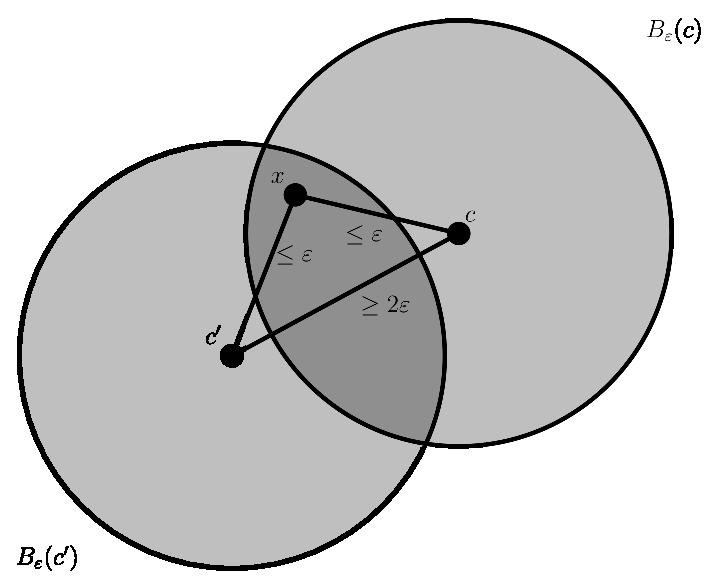
\includegraphics[scale = 0.5]{Figures/chapter1/sphere_packing.eps}
  \caption{If a message $x$ is received with error has distance at most $\e$
  from two codewords $c$ and $c'$, then we cannot reliably decode $x$ into the
  correct codeword that was transmitted.}
  \label{figure_1.1}
\end{figure}

\begin{figure}[h]
  \centering
  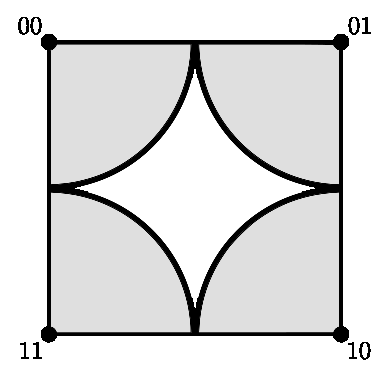
\includegraphics[scale = 0.5]{Figures/chapter1/hamming_box.eps}
  \caption{Arrange the following code $\{00, 01, 10, 11\}$ into a box as shown
  above. Observe that the sphere packing radius for this code is $1$. Now, if
  $x$ is a recieved word with distance at most $1$ to any one (and exactly one)
  of the codewords, then $x$ can be corrected to that codeword. However, if $x$
  differs in more than one spot, we may not be able to determine the original
  transmitted word.}
  \label{figure_1.2}
\end{figure}

\begin{definition}
  Let $Q$ be an alphabet and  $C \subseteq Q^n$ a block code. We define the
  \textbf{covering radius} of $C$ to be the smallest such postivie integer $\r$
  for which that closed balls $B_\r(c)$ cover $Q^n$ for all  $c \in C$; i.e.:
  \begin{equation*}
    Q^n \subseteq \bigcup_{c \in C}{B_\r(c)}
  \end{equation*}
\end{definition}

\begin{lemma}\label{1.1.3}
  Let $C \subseteq Q^n$ a block code, with covering radius $\r$. Then:
  \begin{equation}\label{equation_1.5}
    \r=\max{ \{ \min\{ d(x,y) : c \in C\} : x \in Q^n \} }
  \end{equation}
\end{lemma}
\begin{proof}
   Now, let $x \in Q^n$, and let $c \in C$ for which $x \in B_{\r_{\a_1}}(c)$,
  choose another $c' \in C$ for which $x \in B_{\r_{\a_2}}(c')$. Then we observe
  that $d(x,c) \leq \r_{\a_1}$ and $d(x,c') \leq \r_{\a_2}$. Now, let
  \begin{equation*}
    S_x=\{\r_{\a_i} : d(x,c) \leq \r_{\a_i} \text{ for all } c \in C\}
  \end{equation*}
  and take $\r_\a(x)=\sup{S_x}$. Such a $\r_\a(x)$ exists since each $r_{\a_i}$
  is a positive integer. Then observe that $\r=\inf_{x \in Q^n}{\{\r_\a(x)\}}$.
  This gives us equation \ref{equation_1.5}.
\end{proof}

\begin{figure}[h]
  \centering
  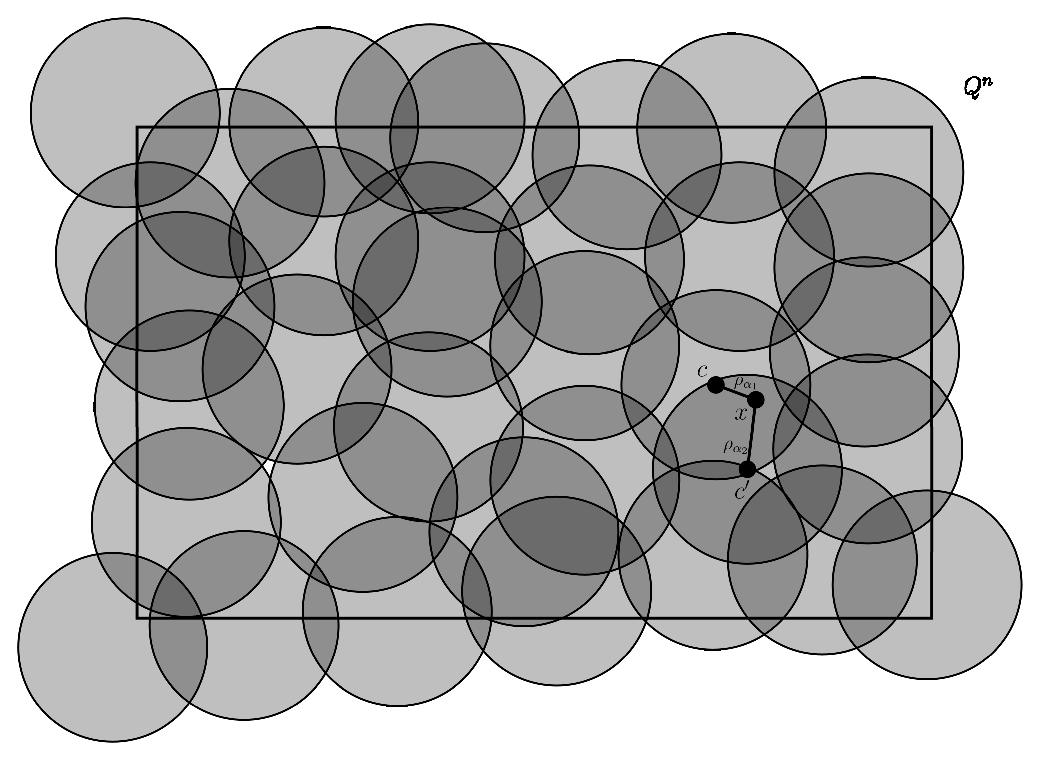
\includegraphics[scale = 0.5]{Figures/chapter1/covering_radius.eps}
  \caption{The covering radius of a code $C$.}
  \label{figure_1.3}
\end{figure}

\begin{definition}
  We call a block code $C$ \textbf{perfect} if its sphere packing radius
  coincides with its covering radius.
\end{definition}

\begin{example}\label{example_1.3}
  The trivial code $C$ of length $n$ in any alphabet is a perfect code, however,
  nothing can be said about the minimum distance of $C$.
\end{example}

\begin{theorem}[The Sphere Packing Bound]\label{theorem_1.1.4}
  Let $C$ be an $\e$-error correcting block code of length $n$ on an alphabet
  $Q$ of size  $q$. Then:
  \begin{equation}\label{equation_1.6}
    |C|\sum_{i=0}^\e{{n \choose i}(q-1)^i} \leq q^n
  \end{equation}
\end{theorem}
\begin{proof}
  If $|Q|=q$, then $|Q^n|=q^n$. Now, let $c \in C$ and choose an $x \in B_\e(c)$
  distinct from $c$. Then $x$ and $c$ differ in  $i \leq \e$ positions. Now,
  since $x \in Q^n$, there are exactly ${n \choose i}$ positions in which $x$
  can differ from $c$, and $q-1$ possible values for $x$. Hence we get that
  \begin{equation*}
    |B_\e(c)|=\sum_{i=1}^\e{ {n \choose i}(q-1)^i }
  \end{equation*}
  Since there are $|C|$ possible codewords, and $q^n$ possible values for $x$ we
  get equation \ref{equation_1.6}
\end{proof}
\begin{corollary}[The Sphere Packing Condition]
  If $C$ is a perfect code, then equality in the sphere packing bound is
  attained. Moreover, the minimum distance of $C$ is exactly $d=2\e+1$.
\end{corollary}
\begin{proof}
  Since $C$ is perfect, by definition, $\e$ is also the covering radius of
  $Q^n$, and we get that $\{B_\e(c)\}$ is a disjoint cover of $Q^n$, hence there
  are no repeated elements in the union $\bigcup{B_\e(c)}$. Then we get:
  \begin{equation*}
    q^n \leq |C|\sum_{i=1}^\e{ {n \choose i}(q-1)^i }
  \end{equation*}
  and equality in the sphere packing bound is attained. This also implies that
  $d \leq 2\e+1$, where $d$ is the minimum distance.
\end{proof}
